\section{Results}
\label{sec:results}

The model is now applied to an anode and a cathode of a high-intensity arc in argon at atmospheric pressure. The two base cases differ in the bulk-plasma state at \(x=L\), in the current density and in electron emission (table~\ref{tab:base}). Unlike the validation cases of Section~\ref{sec:validation}, the radial loss~(\ref{eq:radial-loss}) is included, with the reactive conductivity in the electron channel. The calibration~(\ref{eq:radial-calibration}) gives a column radius \(R=2.3\)~mm for the anode and \(0.42\)~mm for the cathode. At the anode bulk temperature, \(\kappa_R=0.59\ \mathrm{W\,m^{-1}\,K^{-1}}\) is comparable to \(\kappa_e=0.76\ \mathrm{W\,m^{-1}\,K^{-1}}\), whereas at 21\,000~K the plasma is almost fully ionized and \(\kappa_R=0.03\ \mathrm{W\,m^{-1}\,K^{-1}}\) is negligible. At \(x=L\) all densities and temperatures are Dirichlet values (Section~\ref{sec:model-bc}). The anode surface temperature is prescribed, \(T_{\rm wall}=1000\)~K. The cathode surface temperature is not prescribed: it follows from the heat balance~(\ref{eq:bc-heat-balance}), with \(k_w=100\ \mathrm{W\,m^{-1}\,K^{-1}}\), \(L_w=1\)~cm and \(T_0=1000\)~K. The electrode material has \(W=2.63\)~eV and \(A_R=3\times10^4\ \mathrm{A\,m^{-2}\,K^{-2}}\). The domain, grid and refinement are those of Section~\ref{sec:validation}. Each case was integrated in time at fixed current density until the relative change of every variable over \(1\ \mu\)s fell below \(10^{-3}\). In both steady states, the sum of the terms of the electron energy equation~(\ref{eq:eenergy}), i.e.\ \(\partial\mathcal{E}/\partial t\), is below \(1.2\times10^{-3}\) of its largest term everywhere, and the total current density is uniform to within \(10^{-8}\).
% Run record (not for the paper): PlasmeX runs/base_case_anode/plt47000 (BDF2, steady at
% t = 46.6 us) and runs/base_case_cathode/plt01584 (backward-Euler pseudo-transient to t = 1 ms;
% relative change ~1e-5 per us at the end), 11 Oct 2026. Both with prob.use_radial_loss = 4
% (Q_e = Lambda (k_e + k_R(T_e))(T_e - T_edge), k_R the Mutation++ LTE table), Dirichlet arc face
% (arc_len_E = 0, arc_len_Theta = 1e-9, plasmex.heavy_arc_bc = 0). The 9 Oct runs without the
% radial loss are in each run directory's no_radial_loss/ (their numbers in
% figures/results_fig/report_no_radial_loss.txt); the older mode-1 runs in radial_loss_on/.
% Figures and the table's numbers: figures/results_fig/base_case.py (output in report.txt).

\begin{table}[!htbp]
\caption{Base cases: conditions (top) and computed electrode quantities (bottom). The sheath edge \(x_{\rm s}\) is the distance from the electrode at which \(|n_i-n_e|/n_i\) falls to \(1\,\%\), and \(\phi_{\rm s}\) is the potential there; \(\phi(L)\) is the potential at the bulk-plasma boundary. Both potentials are relative to the electrode. Fluxes are towards the electrode.}
\label{tab:base}
\centering
\small
\begin{tabular}{lcc}
\hline
 & Anode & Cathode \\
\hline
Current density \(|J_{\rm app}|\) (\(\mathrm{A\,m^{-2}}\)) & \(9\times10^{6}\) & \(1.2\times10^{8}\) \\
Bulk temperature \(T_{\rm bulk}\) (K) & 12\,400 & 21\,000 \\
Bulk electron density \(n_e^{\rm bulk}\) (\(\mathrm{m^{-3}}\)) & \(8.2\times10^{22}\) & \(1.7\times10^{23}\) \\
Thermionic emission & off & on \\
\hline
Surface temperature \(T_{\rm wall}\) (K) & 1000 (prescribed) & 3698 \\
\(T_e\) at the surface (K) & 4900 & 19\,500 \\
\(n_e\), \(n_i\) at the surface (\(\mathrm{m^{-3}}\)) & \(5.2\times10^{20}\), \(4.7\times10^{20}\) & \(2.1\times10^{21}\), \(7.6\times10^{21}\) \\
Sheath edge, \(x_{\rm s}\) (m) & \(8.4\times10^{-7}\) & \(5.7\times10^{-7}\) \\
\(\phi_{\rm s}\), \(\phi(L)\) (V) & 0.41, 2.60 & 4.13, 13.68 \\
Field at the surface (\(\mathrm{V\,m^{-1}}\)) & \(-7.2\times10^{5}\) & \(2.2\times10^{7}\) \\
\(j_i/j\) at the surface & \(-0.0037\) & 0.057 \\
Absorbed electron flux \(\tfrac14n_e\bar c_e\) (\(\mathrm{m^{-2}\,s^{-1}}\)) & \(5.6\times10^{25}\) & \(4.6\times10^{26}\) \\
Emitted electron flux \(\Gamma_{\rm em}\) (\(\mathrm{m^{-2}\,s^{-1}}\)) & -- & \(1.17\times10^{27}\) \\
Ion flux \(\boldsymbol{\Gamma}_i\cdot\hat{\mathbf{n}}\) (\(\mathrm{m^{-2}\,s^{-1}}\)) & \(2.1\times10^{23}\) & \(4.3\times10^{25}\) \\
Heat flux \(q_w\) (\(\mathrm{MW\,m^{-2}}\)) & 38.2 & 27.0 \\
\hline
\end{tabular}
\end{table}

\begin{figure}[p]
\centering
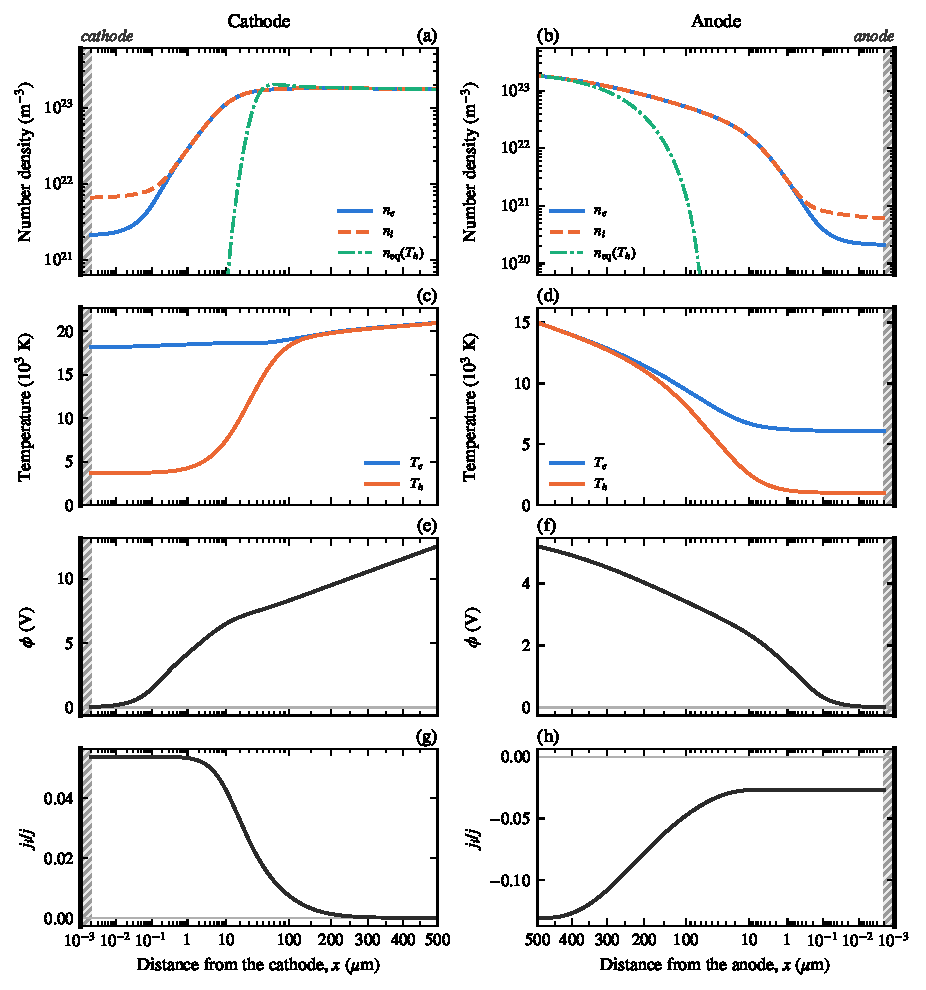
\includegraphics[width=0.92\textwidth]{figures/results_fig/base_profiles.pdf}
\caption{Base cases: cathode (left) and anode (right). \(x\) is the distance from the electrode; the cathode surface is at the left edge of its panels and the anode surface at the right edge of its panels, marked by the hatched strip. The distance axis is scaled as \(\ln x+x/x_c\), with \(x_c=50\ \mu\)m: logarithmic near the electrode and smoothly becoming linear towards the bulk plasma, so that both the sheath and the approach to the bulk are visible. (a), (b) Electron, ion and atom number densities. (c), (d) Electron and heavy-particle temperatures, and the effective ion temperature \(T_{\rm eff}\) of the two-temperature ion mobility (Appendix~\ref{app:transport}), shown where \(n_n>n_i\), the range in which the ion--atom closure applies. (e), (f) Potential relative to the electrode. (g), (h) Ion fraction of the current density, positive for ions flowing into the electrode.}
\label{fig:base-profiles}
\end{figure}

\subsection{Structure of the near-electrode layers}
\label{sec:res-structure}

Figure~\ref{fig:base-profiles} shows the steady profiles of both cases. In both, the plasma departs from LTE over a layer of order \(10^{-4}\)~m, as estimated in Section~\ref{sec:model-governing}, but the structure of this layer is very different at the two electrodes.

\emph{Anode.} The space-charge sheath is practically absent. Charge separation exceeds 1\,\% only within \(0.84\ \mu\)m of the surface, where the potential differs from that of the anode by 0.41~V, and at the surface \(n_e\) exceeds \(n_i\) by 9\,\% (figure~\ref{fig:base-profiles}(b)). The anode lies 2.60~V below the bulk-plasma boundary, and this drop is distributed over the whole quasi-neutral layer (figure~\ref{fig:base-profiles}(f)): 1.14~V within \(10\ \mu\)m, 1.83~V within \(100\ \mu\)m. The field is directed towards the anode and retards the electrons, which reach the surface by diffusion down the steep density gradient: the charged-particle density falls by a factor of 160, from \(8.2\times10^{22}\) to \(5.2\times10^{20}\ \mathrm{m^{-3}}\), across the layer. The electron and heavy-particle temperatures decrease together towards the anode, but \(T_h\) falls faster, to the prescribed surface temperature of 1~kK, so that the two separate progressively: by 2.1~kK at \(x=10^{-4}\)~m, 3.6~kK at \(x=10^{-5}\)~m, and 3.9~kK at the surface, where \(T_e=4.9\)~kK (figure~\ref{fig:base-profiles}(d)). Ions flow into the anode, \(j_i/j<0\), and carry only 0.4\,\% of the current at the surface (figure~\ref{fig:base-profiles}(h)). The field at the anode, \(7.2\times10^5\ \mathrm{V\,m^{-1}}\), is too weak to heat the ions: \(T_{\rm eff}\) exceeds \(T_h\) by about 0.1~kK.

\emph{Cathode.} A space-charge sheath forms, \(0.57\ \mu\)m thick, in which \(n_i\) exceeds \(n_e\) by up to a factor of 3.6 at the surface (figure~\ref{fig:base-profiles}(a)), and across which the potential rises by 4.1~V. The field at the surface is \(2.2\times10^7\ \mathrm{V\,m^{-1}}\). Beyond the sheath, the potential keeps rising through the quasi-neutral ionization layer, to 8.8~V at \(x=10^{-4}\)~m (figure~\ref{fig:base-profiles}(e)). Further out, the plasma approaches the bulk state, and the remaining rise to 13.7~V at \(x=L\) is mostly the ohmic drop of the column, whose field is \(1.1\times10^4\ \mathrm{V\,m^{-1}}\). The electron temperature is nearly uniform, 19.5--21~kK, across the whole layer, while the heavy-particle temperature rises from the surface value of 3.7~kK and approaches \(T_e\) only at \(x\approx10^{-4}\)~m (figure~\ref{fig:base-profiles}(c)). Over the same distance the atom density falls by three orders of magnitude, from \(2\times10^{24}\) to \(2.6\times10^{22}\ \mathrm{m^{-3}}\), and the plasma becomes almost fully ionized. The emitted electron flux, \(1.17\times10^{27}\ \mathrm{m^{-2}\,s^{-1}}\), corresponds to a current density of \(1.9\times10^8\ \mathrm{A\,m^{-2}}\), larger than the arc current density. It is partly returned by the plasma electrons that reach the surface against the sheath field, \(4.6\times10^{26}\ \mathrm{m^{-2}\,s^{-1}}\) (table~\ref{tab:base}), and the ions carry 5.7\,\% of the current at the surface (figure~\ref{fig:base-profiles}(g)). In the sheath, the ions are strongly heated by the field: \(T_{\rm eff}\) reaches 48~kK at the surface (figure~\ref{fig:base-profiles}(c)).

\begin{figure}[!htbp]
\centering
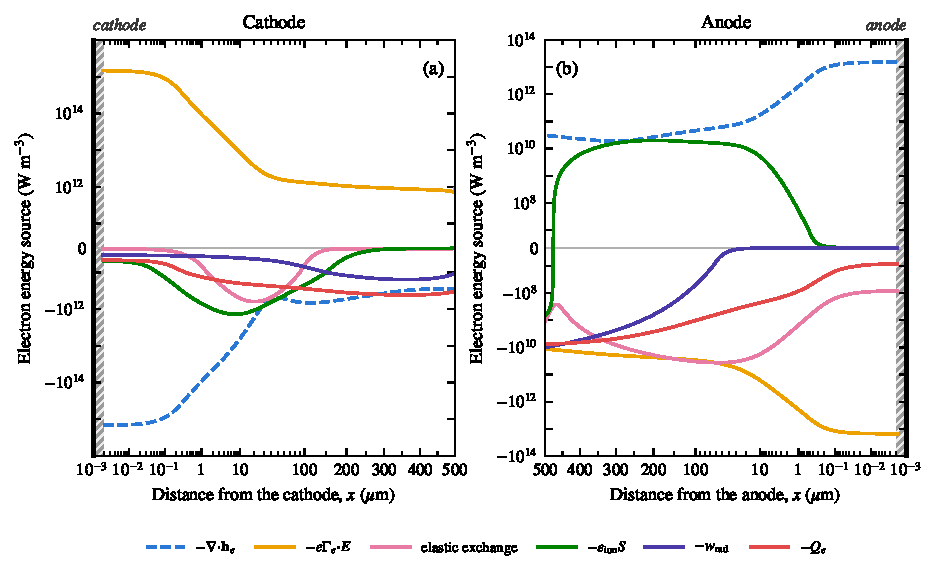
\includegraphics[width=\textwidth]{figures/results_fig/base_een_budget.pdf}
\caption{Steady electron energy balance, equation~(\ref{eq:eenergy}), for (a) the cathode and (b) the anode: every term except \(\partial\mathcal{E}/\partial t\). Dashed: the divergence of the electron energy flux~(\ref{eq:heatflux-e}), \(-\nabla\cdot\mathbf{h}_e\). Solid: the volume terms, i.e.\ Joule heating, elastic exchange with the heavy particles, the ionization sink and the radiative loss. Positive terms heat the electrons. The hatched strip marks the electrode surface: the cathode at the left of panel (a), the anode at the right of panel (b). The distance axis is scaled as \(\ln x+x/x_c\), with \(x_c=50\ \mu\)m: logarithmic near the electrode and smoothly becoming linear towards the bulk plasma, so that both the sheath and the approach to the bulk are visible. The vertical axis is logarithmic in \(|\cdot|\) above \(10^{11}\) (a) and \(10^{6}\ \mathrm{W\,m^{-3}}\) (b), and linear below.}
\label{fig:base-budget}
\end{figure}

\subsection{Electron energy balance}
\label{sec:res-energy}

Figure~\ref{fig:base-budget} compares the terms of the electron energy equation~(\ref{eq:eenergy}) across the layer. The ordering of the terms is again opposite at the two electrodes.

\emph{Anode.} The Joule term \(-e\boldsymbol{\Gamma}_e\cdot\mathbf{E}\) is negative throughout the layer (figure~\ref{fig:base-budget}(b)): the electrons flow towards the anode against the retarding field and lose energy to it, \(23.5\ \mathrm{MW\,m^{-2}}\) over the domain. This loss, and the smaller elastic (\(4.5\ \mathrm{MW\,m^{-2}}\)) and radial (\(2.6\ \mathrm{MW\,m^{-2}}\)) losses, are supplied by the electron energy flux from the column. At \(x=L\), \(36.4\ \mathrm{MW\,m^{-2}}\) flow towards the anode, two thirds of it as the enthalpy flux \(\tfrac52k_BT_e\boldsymbol{\Gamma}_e\), and only \(7.6\ \mathrm{MW\,m^{-2}}\) reach the surface. The convergence of the enthalpy flux, as \(T_e\) falls towards the anode, supplies \(15.0\ \mathrm{MW\,m^{-2}}\), conduction \(4.2\ \mathrm{MW\,m^{-2}}\) and the thermal-diffusion heat flux \(9.6\ \mathrm{MW\,m^{-2}}\). Close to the anode, \(x<10\ \mu\)m, conduction and thermal diffusion provide almost all of the supply, and within \(0.1\ \mu\)m of the surface the thermal-diffusion term alone balances the Joule loss. The volume exchange terms are smaller than the flux terms by two to three orders of magnitude near the anode, and become comparable to them only at \(x\gtrsim10^{-4}\)~m, where the elastic loss to the heavy particles keeps \(T_h\) close to \(T_e\). The ionization term is positive over most of the layer: near the anode the plasma recombines, \(S<0\), because the charged particles are supplied by diffusion at densities well above the local ionization equilibrium (Section~\ref{sec:val-anode}), and the recombination energy heats the electrons.

\emph{Cathode.} Joule heating is the dominant electron energy source everywhere in the layer (figure~\ref{fig:base-budget}(a)). It reaches \(2.5\times10^{15}\ \mathrm{W\,m^{-3}}\) at the surface, where the emitted electrons are accelerated by the sheath field. \(467\ \mathrm{MW\,m^{-2}}\) are deposited in the sheath, and \(1590\ \mathrm{MW\,m^{-2}}\) over the whole domain. In the sheath, the Joule heating is balanced by the divergence of the conduction and thermal-diffusion fluxes (\(334\) and \(113\ \mathrm{MW\,m^{-2}}\)). The electron temperature is slightly lower at the surface than at the sheath edge, 19.5 against 19.7~kK, so these fluxes carry heat towards the cathode. The enthalpy flux of the electron current, directed away from the cathode, is large, 480--540~\(\mathrm{MW\,m^{-2}}\), but nearly uniform, and its divergence is an order of magnitude smaller than that of conduction. Conduction changes sign at \(x\approx1.4\times10^{-5}\)~m and deposits energy in the ionization layer, out to \(x\approx10^{-4}\)~m, where ionization (\(98\ \mathrm{MW\,m^{-2}}\) within \(100\ \mu\)m) and the elastic heating of the heavy particles take it up. Over the whole domain, the Joule heat is distributed as follows: \(690\ \mathrm{MW\,m^{-2}}\) leave at \(x=L\) as electron energy flux into the column (\(543\ \mathrm{MW\,m^{-2}}\) of enthalpy and \(153\ \mathrm{MW\,m^{-2}}\) of thermal-diffusion heat flux); \(574\ \mathrm{MW\,m^{-2}}\) are radial loss, most of it in the column part of the domain, \(x>10^{-4}\)~m; \(130\ \mathrm{MW\,m^{-2}}\) reach the cathode with the absorbed plasma electrons, net of the energy of the emitted electrons; ionization takes \(108\ \mathrm{MW\,m^{-2}}\); and radiation and elastic exchange take \(46\) and \(44\ \mathrm{MW\,m^{-2}}\).

\begin{figure}[!htbp]
\centering
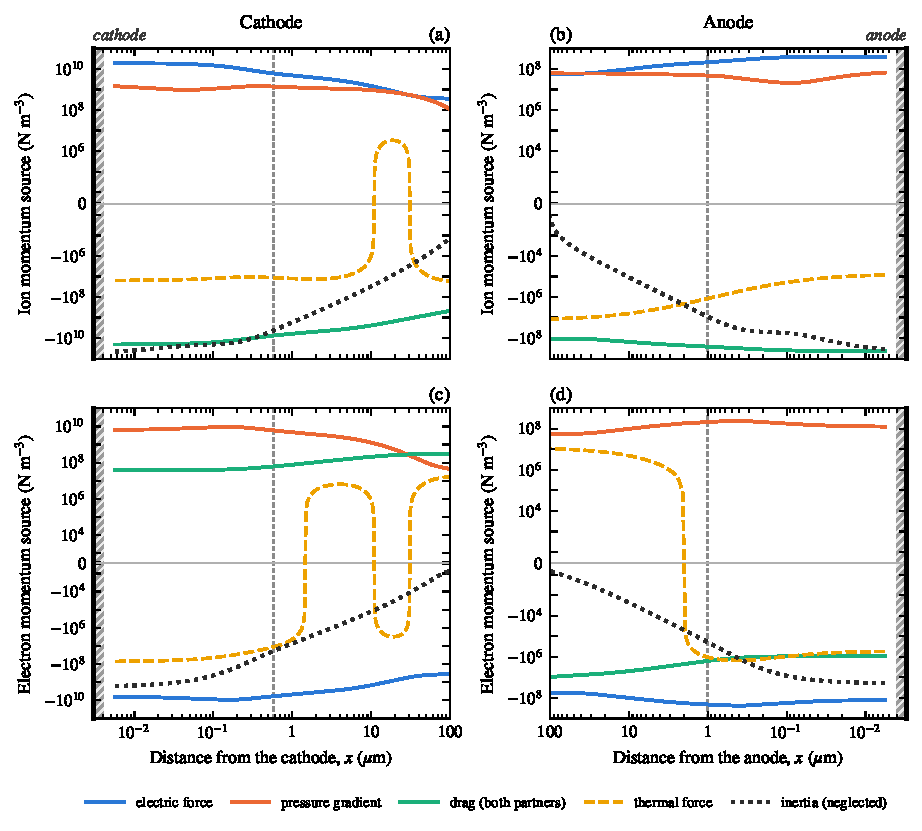
\includegraphics[width=\textwidth]{figures/results_fig/base_momentum.pdf}
\caption{Terms of the steady momentum balances of the ions, equation~(\ref{eq:mom-i}), (a) and (b), and of the electrons, equation~(\ref{eq:mom-e}), (c) and (d), at the cathode (left) and the anode (right), within \(100\ \mu\)m of the electrode. Positive terms push the species towards the electrode. Drag: the friction with both collision partners combined; thermal force: the term in \(C_e\) of equation~(\ref{eq:mom-e}) and its reaction \(C_i\) on the ions. Dotted: the inertia \(-m_sn_s(\mathbf{u}_s\cdot\nabla)\mathbf{u}_s\), which the model neglects, evaluated with \(\mathbf{u}_s=\boldsymbol{\Gamma}_s/n_s\) from the computed fluxes. The vertical dashed line marks the sheath edge \(x_{\rm s}\) (table~\ref{tab:base}). The vertical axis is logarithmic in \(|\cdot|\) and linear within six decades of the largest term.}
\label{fig:base-momentum}
\end{figure}

\begin{figure}[!htbp]
\centering
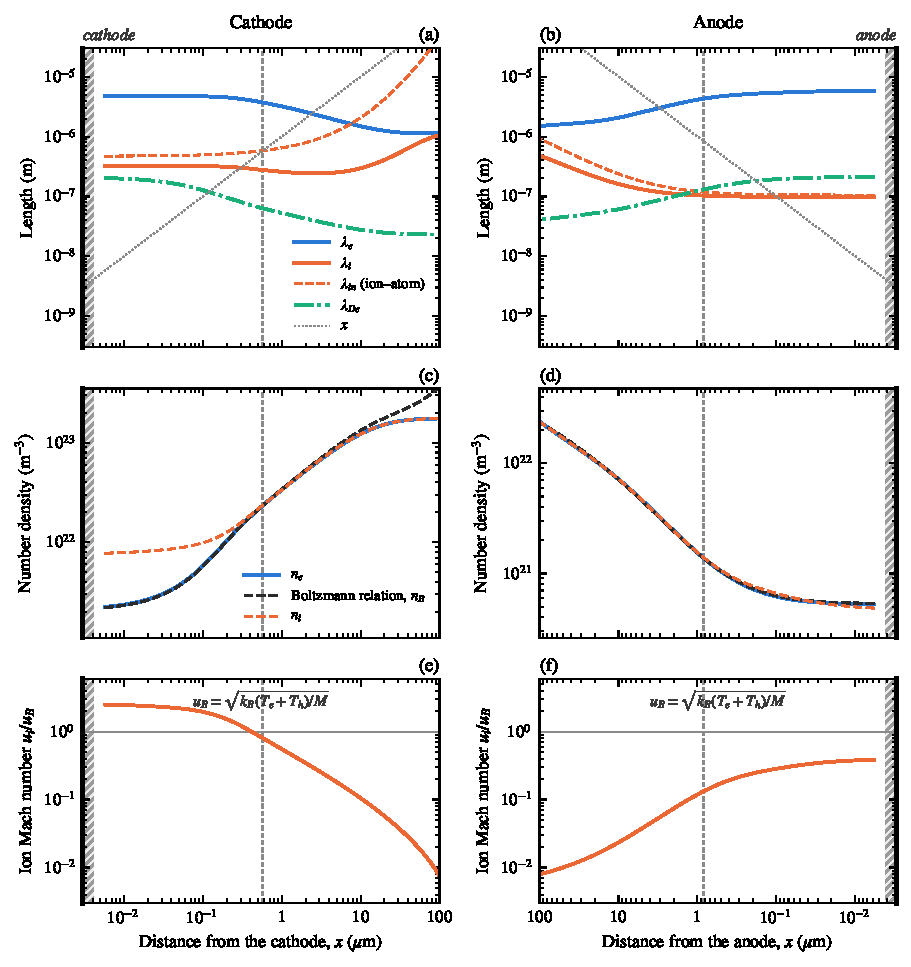
\includegraphics[width=0.92\textwidth]{figures/results_fig/base_sheath.pdf}
\caption{The sheaths of the base cases: cathode (left) and anode (right). (a), (b) Electron and ion mean free paths, the ion--atom part of the latter, and the electron Debye length, from the local state; dotted: the distance \(x\) from the electrode. (c), (d) Electron density and the Boltzmann relation \(n_B=n_e(x_{\rm s})\exp[(e/k_B)\int_{\phi_{\rm s}}^{\phi}d\phi'/T_e]\) started at the sheath edge, with the ion density for reference. (e), (f) Ion velocity towards the electrode, \(u_i=\Gamma_i/n_i\), relative to the Bohm velocity \(u_B=\sqrt{k_B(T_e+T_h)/M}\). The vertical dashed line marks the sheath edge \(x_{\rm s}\).}
\label{fig:base-sheath}
\end{figure}

\subsection{Momentum balance and collisionality of the sheaths}
\label{sec:res-momentum}
% Figures and numbers: figures/results_fig/base_sheath.py (output in base_sheath_report.txt), same plotfiles.

The fluxes~(\ref{eq:flux-e}) and (\ref{eq:flux-i}) follow from the force balances~(\ref{eq:mom-e}) and (\ref{eq:mom-i}), in which the inertia of each species relative to the heavy gas is neglected. Figure~\ref{fig:base-momentum} shows the terms of these balances in the two steady states near the electrode: the electric force, the pressure gradient, the two collisional drags combined, and the thermal force. In the steady states the heavy gas is at rest (\(|\mathbf{u}|\le4\times10^{-4}\ \mathrm{m\,s^{-1}}\) at the cathode and \(0.16\ \mathrm{m\,s^{-1}}\) at the anode), so the share \(Y_s\mathbf{F}\) of the net force is negligible (below \(2\times10^{-4}\) of the largest term). For comparison, the figure also shows the inertia \(m_sn_s(\mathbf{u}_s\cdot\nabla)\mathbf{u}_s\) that the model neglects, evaluated a posteriori from the computed fluxes. The retained terms sum to zero to within \(3\times10^{-3}\) of the largest one.

\emph{Ions.} In both sheaths, the electric force on the ions is balanced by the drag (figure~\ref{fig:base-momentum}(a), (b)). At the cathode the pressure gradient adds at most 22\,\% to the electric force in the sheath, and 7\,\% at the surface. At the anode the field is weaker, and the pressure gradient, which also drives the ions towards the surface, is 68\,\% of the electric force there. The thermal force on the ions is negligible, below 1\,\% of the drag in either sheath. The neglected inertia is not small inside the cathode sheath. It exceeds the drag within \(0.36\ \mu\)m of the surface, by a factor of 2.4 at the surface, and stays above 10\,\% of the drag out to \(2.3\ \mu\)m; beyond \(14\ \mu\)m it is below 1\,\%. At the anode the inertia is at most 35\,\% of the drag, at the surface, and below 10\,\% beyond \(0.09\ \mu\)m.

\emph{Electrons.} In both sheaths the field retards the electrons, and the electric force on them is balanced by their pressure gradient (figure~\ref{fig:base-momentum}(c), (d)). In the sheath the two cancel to within 0.9\,\% (cathode) and 4.7\,\% (anode) of the electric force. The drag (0.6 and 2.6\,\% of the electric force at the surface) and the thermal force (1.2 and 0.9\,\%) are small there. The drag becomes important only in the quasi-neutral layer, where it carries the current: at \(10\ \mu\)m from the surface it is 16\,\% (cathode) and 20\,\% (anode) of the electric force. The inertia of the electrons exceeds their drag within \(0.33\ \mu\)m of the cathode (by up to a factor of 54) and within \(0.59\ \mu\)m of the anode (by up to a factor of 6), but it remains smaller than the electric force: at the surface it is a third of the electric force at the cathode and 16\,\% at the anode, and at the sheath edge 0.3 and 2.3\,\%. At the cathode, this inertia is that of the emitted electrons, accelerated by the sheath field.

\emph{Mean free paths.} Figure~\ref{fig:base-sheath}(a), (b) shows the mean free paths \(\lambda_e\) and \(\lambda_i\) of table~\ref{tab:scales}, evaluated with the local densities and temperatures, the ion--atom part of \(\lambda_i\), \(\lambda_{in}=1/(n_n\overline{Q}_{in})\), and the electron Debye length. The electron mean free path is of order microns, \(3.8\ \mu\)m at the cathode sheath edge and \(4.3\ \mu\)m at the anode one. The sheaths, \(0.57\) and \(0.84\ \mu\)m thick, therefore contain only 0.13 and 0.17 electron mean free paths, and \(\lambda_e\) exceeds the distance from the surface within \(2.3\ \mu\)m of the cathode and \(2.8\ \mu\)m of the anode. The ions are more collisional. At the sheath edge, \(\lambda_i=0.28\ \mu\)m at the cathode and \(0.10\ \mu\)m at the anode, so that the ions cross 1.8 and 8.2 mean free paths in the sheaths (1.05 and 7.4 counting only the collisions with atoms). The anode sheath is thus collision-dominated for the ions, consistent with their small inertia. The cathode sheath is transitional: the ions make one to two collisions across it, and their inertia exceeds the drag over its inner two thirds. There the ions cannot follow the steep rise of the field, and the local relation between field and ion velocity in equation~(\ref{eq:flux-i}) overestimates the ion velocity near the surface. The electrons cross both sheaths practically without collisions. Their balance there is, however, not a balance of collisional transport: the drag is a few per cent of the electric force, and the field and pressure gradient balance each other as in the Boltzmann equilibrium of a Maxwellian population retarded by a potential barrier, which does not require collisions. The electron description therefore remains adequate in the sheaths, except within about \(0.1\ \mu\)m of the cathode, where the inertia of the emitted electrons is no longer small. Beyond 2--3~\(\mu\)m from either electrode, the inertia of both species is below 10\,\% of the drag, and the inertialess, collision-dominated description of section~\ref{sec:model-governing} holds.

\emph{Boltzmann electrons and the Bohm criterion.} Simplified sheath models describe the electrons in the sheath by the Boltzmann relation and impose the Bohm criterion on the ions entering it, \(u_i\ge u_B\), with \(u_B=\sqrt{k_B(T_e+T_i)/M}\). Figure~\ref{fig:base-sheath}(c)--(f) tests both against the computed sheaths. The electron density follows the Boltzmann relation closely. Started at the sheath edge, the relation reproduces \(n_e\) to within 1.5\,\% across the cathode sheath, where \(n_e\) falls by a factor of 10, and to within 2.1\,\% across the anode sheath, where it falls by a factor of 2.6. Outside the anode sheath it still holds to within 2.3\,\% at \(100\ \mu\)m. At the cathode it fails progressively in the ionization layer, where the electron drag carries the current: \(n_e\) is 8\,\% below \(n_B\) at \(10\ \mu\)m and 53\,\% below at \(100\ \mu\)m. The ions, in contrast, do not satisfy the Bohm criterion at the sheath edge (figure~\ref{fig:base-sheath}(e), (f)). At the cathode they enter the sheath at \(u_i=1830\ \mathrm{m\,s^{-1}}\), against \(u_B=2230\ \mathrm{m\,s^{-1}}\), i.e.\ at 0.82\,\(u_B\). They reach \(u_B\) only \(0.40\ \mu\)m from the surface, inside the sheath, where the charge separation is already 2.9\,\%, and arrive at the surface at 2.5\,\(u_B\). At the anode the ions enter the sheath at 0.13\,\(u_B\) and reach the surface at 0.39\,\(u_B\), never attaining \(u_B\). The Bohm flux \(n_iu_B\) at the sheath edge would therefore overestimate the ion flux entering the sheath by 22\,\% at the cathode and by a factor of 7.5 at the anode. The Bohm criterion is derived for a collisionless sheath. In these sheaths the ions collide with the atoms throughout the presheath and the sheath, and, except in the inner part of the cathode sheath, their velocity is set by the balance of the electric force and the drag rather than by the potential drop they have fallen through. This agrees with the conclusion of Semenov et al.\ \cite{semenov2016numerical} for the anode layer.

\begin{figure}[!htbp]
\centering
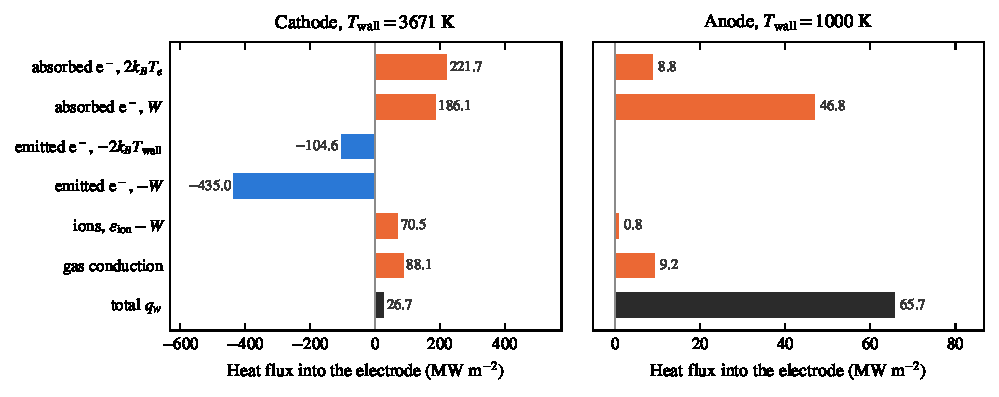
\includegraphics[width=\textwidth]{figures/results_fig/base_qwall.pdf}
\caption{Terms of the heat flux delivered to the electrode, equation~(\ref{eq:bc-qwall}), positive into the electrode, for the cathode (left) and the anode (right). Orange: heating; blue: emission cooling; black: the net heat flux \(q_w\). At the cathode, \(q_w\) equals the conduction \(k_w(T_{\rm wall}-T_0)/L_w\) into the electrode body, equation~(\ref{eq:bc-heat-balance}); the anode surface temperature is prescribed.}
\label{fig:base-qwall}
\end{figure}

\subsection{Heat flux to the electrode}
\label{sec:res-heat}

The terms of the electrode heat flux~(\ref{eq:bc-qwall}) are shown in figure~\ref{fig:base-qwall}. At the anode, \(q_w=38.2\ \mathrm{MW\,m^{-2}}\) and the absorbed electrons deliver 82\,\% of it: 23.8~\(\mathrm{MW\,m^{-2}}\) as the work function released on entering the metal and 7.6~\(\mathrm{MW\,m^{-2}}\) as kinetic energy. Gas conduction contributes \(6.4\ \mathrm{MW\,m^{-2}}\) and ion recombination about 1\,\%. The anode heat flux is thus set by the electron current, through \(W\), and by the electron temperature at the surface; with the surface temperature prescribed, it is the heat that the anode cooling has to remove.

At the cathode, the heat flux is the small difference of large terms. The absorbed plasma electrons (\(443\ \mathrm{MW\,m^{-2}}\)), gas conduction (\(105\ \mathrm{MW\,m^{-2}}\)) and ion recombination (\(90\ \mathrm{MW\,m^{-2}}\)) heat the surface by \(638\ \mathrm{MW\,m^{-2}}\) in total, and emission cools it by \(611\ \mathrm{MW\,m^{-2}}\), so that only \(q_w=27.0\ \mathrm{MW\,m^{-2}}\) is conducted into the cathode body. The surface temperature, 3698~K, is therefore fixed mainly by the condition that emission cooling nearly balances the heating, and only weakly by the conduction into the cathode body. Emission cooling grows with \(T_{\rm wall}\) as \(T_{\rm wall}^2\exp[-(W-\Delta W)/(k_BT_{\rm wall})]\), i.e.\ by about 0.27\,\% per kelvin at this temperature, so a 5\,\% change in the heating would shift \(T_{\rm wall}\) by only about 20~K, and \(q_w\) by less than 1\,\%. Ion recombination, at \(\varepsilon_{\rm ion}-W=13.1\)~eV per ion, provides 14\,\% of the heating, although the ions carry only 5.7\,\% of the current.

\emph{Ion impact energy.} Equation~(\ref{eq:bc-qwall}) charges the ions with their recombination energy only, not with the kinetic energy with which they strike the surface. In the model, the ion energy follows from the local field through the two-temperature closure (Appendix~\ref{app:transport}), which presumes that the ions make many collisions over the distance in which the field changes. The cathode sheath does not satisfy this: the ions cross it with only one to two collisions, and their inertia exceeds the drag over its inner part (Section~\ref{sec:res-momentum}). The local mean ion energy at the cathode surface is therefore not a reliable impact energy, and its distribution would require a kinetic treatment of the sheath. We therefore give only the maximum impact energy at the cathode: that of an ion that enters the sheath with the mean energy at the sheath edge, \(\tfrac32k_BT_{\rm eff}+\tfrac12Mv_d^2=1.5\)~eV (equations~(\ref{eq:wannier}) and (\ref{eq:mu-in})), and crosses it without a collision, gaining \(e\phi_{\rm s}=4.1\)~eV. This maximum is 5.6~eV per ion, and with the ion flux of table~\ref{tab:base} it delivers at most \(38\ \mathrm{MW\,m^{-2}}\), comparable to \(q_w\) itself. Added to the heating, this term would, however, raise \(T_{\rm wall}\) by only about 20~K, most of it being removed by emission cooling, and \(q_w\) by about 1\,\%. At the anode, where the ions carry 0.4\,\% of the current and fall through only 0.41~V in a collision-dominated sheath, their kinetic energy is negligible.


\subsection{Dependence on the bulk temperature and the current density}
\label{sec:res-sweep}
% Run record (not for the paper): PlasmeX runs/base_sweep, 11 Oct 2026 (launch.sh,
% ladder4_J2e8.sh, tighten_and_1p5.sh; what failed is in failed_attempts/). Every run stopped by
% the steady-state trigger; energy residual <= 1.3e-3 of the largest term. Anode: from the base
% state (plasmex.init_plotfile). Cathode: J = 8e7, 9e7 (from the old cathode_sweep 8e7 state), 1e8
% from a steady state, the T series from the uniform initial state, J > 1.2e8 by a 4 % current
% ladder of checkpoint restarts (prob.wall_temp_tau = 1e-6 s from 1.3e8 on; same steady state).
% Above ~1.5e8 no route reached a steady state; the user ended the sweep at 1.5e8. All cathode
% states restarted at steady_tol = 1e-5 (tight/), so the heat balance closes to 9e-4.
% Figures and numbers: figures/results_fig/base_sweep.py (base_sweep.csv).

The base cases were repeated with the bulk temperature varied at fixed current density, \(T_{\rm bulk}=11\,000\)--\(14\,000\)~K for the anode and \(19\,000\)--\(23\,000\)~K for the cathode (figure~\ref{fig:sweep-T}), and with the current density varied at the base bulk temperature, \(|J_{\rm app}|=7\times10^{6}\)--\(2\times10^{7}\ \mathrm{A\,m^{-2}}\) for the anode and \(8\times10^{7}\)--\(1.5\times10^{8}\ \mathrm{A\,m^{-2}}\) for the cathode (figure~\ref{fig:sweep-J}). Everything else is as in the base cases. In particular, \(\Lambda\) is recalibrated for each bulk state through equation~(\ref{eq:radial-calibration}), which gives column radii of 1.0--4.1~mm for the anode cases and 0.33--0.66~mm for the cathode cases.

\begin{figure}[p]
\centering
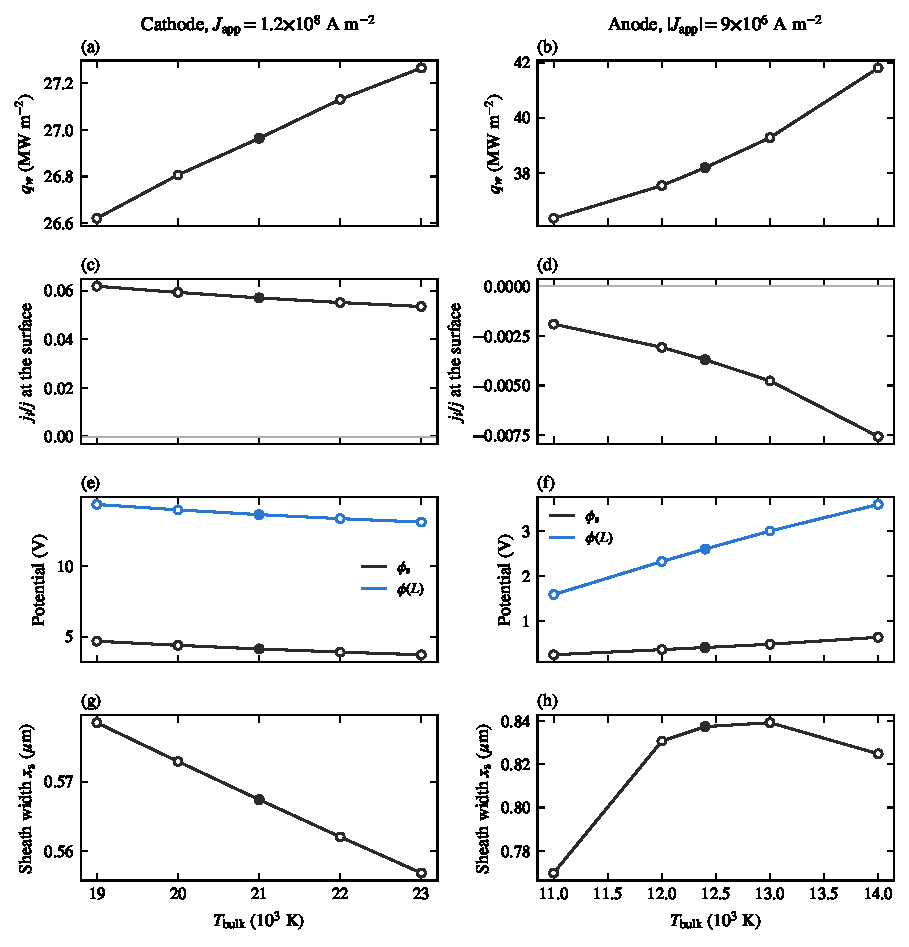
\includegraphics[width=0.92\textwidth]{figures/results_fig/base_sweep_T.pdf}
\caption{Electrode quantities against the bulk temperature \(T_{\rm bulk}\), for the cathode at \(J_{\rm app}=1.2\times10^{8}\ \mathrm{A\,m^{-2}}\) (left) and the anode at \(|J_{\rm app}|=9\times10^{6}\ \mathrm{A\,m^{-2}}\) (right). Filled symbols: the base cases. (a), (b) Heat flux into the electrode \(q_w\), equation~(\ref{eq:bc-qwall}). (c), (d) Ion fraction of the current density at the surface, positive for ions flowing into the cathode; at the anode the ions also flow into the surface, against the current. (e), (f) Potential at the sheath edge \(\phi_{\rm s}\) and at the bulk-plasma boundary \(\phi(L)\), relative to the electrode. (g), (h) Sheath width \(x_{\rm s}\), the distance from the surface at which \(|n_i-n_e|/n_i\) falls to 1\,\%.}
\label{fig:sweep-T}
\end{figure}

\begin{figure}[p]
\centering
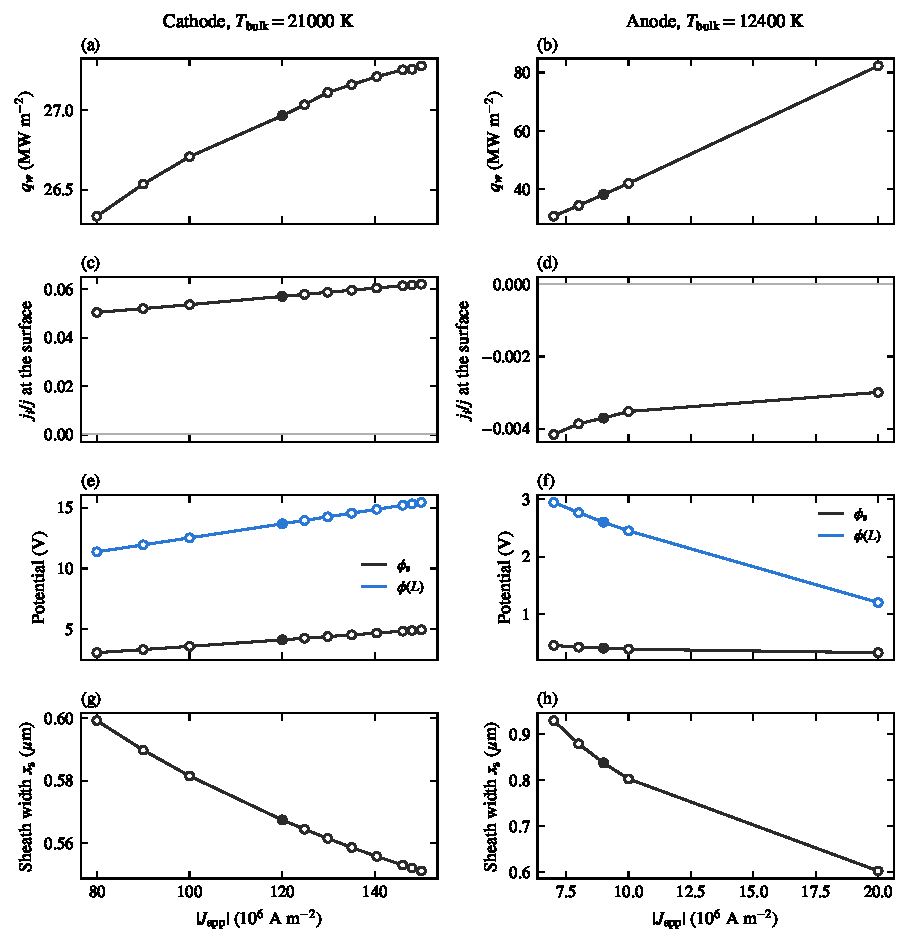
\includegraphics[width=0.92\textwidth]{figures/results_fig/base_sweep_J.pdf}
\caption{As figure~\ref{fig:sweep-T}, against the current density \(|J_{\rm app}|\), for the cathode at \(T_{\rm bulk}=21\,000\)~K (left) and the anode at \(T_{\rm bulk}=12\,400\)~K (right).}
\label{fig:sweep-J}
\end{figure}

\emph{Cathode.} The heat flux to the cathode hardly changes: \(q_w=26.3\)--\(27.3\ \mathrm{MW\,m^{-2}}\) in every case (figures~\ref{fig:sweep-T}(a) and \ref{fig:sweep-J}(a)), while \(T_{\rm wall}\) varies only between 3633 and 3727~K. This follows from the heat balance~(\ref{eq:bc-heat-balance}). With the electrode parameters used here, a change of \(q_w\) by \(1\ \mathrm{MW\,m^{-2}}\) requires a change of \(T_{\rm wall}\) by 100~K, which would change the emission cooling by about 30\,\%. The heating of the surface, by the absorbed electrons, the ions and gas conduction, does depend on the plasma: it increases from 488 to \(735\ \mathrm{MW\,m^{-2}}\) between \(J_{\rm app}=8\times10^{7}\) and \(1.5\times10^{8}\ \mathrm{A\,m^{-2}}\). The surface temperature then rises by only 94~K, and the additional heating is removed by emission cooling. Within these ranges, the heat flux conducted into the cathode is therefore set by the electrode, through \(W\), \(A_R\), \(k_w\), \(L_w\) and \(T_0\), rather than by the plasma. The plasma side adjusts instead. With increasing current density, the sheath drop rises from 3.1 to 5.0~V and the ion fraction of the current at the surface from 5.0 to 6.2\,\% (figure~\ref{fig:sweep-J}). The electron temperature at the surface rises from 16.7 to 21.4~kK, and the voltage across the domain from 11.4 to 15.4~V. The emitted current exceeds the arc current in every case, but by less as the current grows, from 1.77 to 1.44 times the arc current. Above \(1.5\times10^{8}\ \mathrm{A\,m^{-2}}\) no steady state was reached with this cathode heat balance. Increasing the bulk temperature at fixed current acts in the opposite direction on the sheath (figure~\ref{fig:sweep-T}). Between 19\,000 and 23\,000~K, \(\phi_{\rm s}\) decreases from 4.7 to 3.7~V, \(j_i/j\) from 6.2 to 5.3\,\% and \(T_e\) at the surface from 20.3 to 18.9~kK, while the voltage across the domain \(\phi(L)\) falls from 14.4 to 13.1~V. The sheath width changes by less than 10\,\% in either sweep (figures~\ref{fig:sweep-T}(g) and \ref{fig:sweep-J}(g)): it decreases from 0.60 to \(0.55\ \mu\)m as the current density increases, and from 0.58 to \(0.56\ \mu\)m as the bulk temperature increases. The larger sheath drop at higher current is held across a nearly unchanged width by a denser ion space charge: the ion density at the surface rises from \(5.5\times10^{21}\) to \(9.2\times10^{21}\ \mathrm{m^{-3}}\).

\emph{Anode.} The anode heat flux increases almost in proportion to the current density, from 30.7 to \(82.3\ \mathrm{MW\,m^{-2}}\) between \(|J_{\rm app}|=7\times10^{6}\) and \(2\times10^{7}\ \mathrm{A\,m^{-2}}\) (figure~\ref{fig:sweep-J}(b)), i.e.\ 4.4 to 4.1~W per ampere. Of this, the work function released by the absorbed electrons contributes exactly \(W|J_{\rm app}|/e\), i.e.\ 2.63~W per ampere. Their kinetic energy, \(2k_BT_e\) per electron with \(T_e\) at the surface rising from 4.7 to 6.0~kK, contributes another 0.8--1.0~W per ampere. Gas conduction (6.1--\(7.9\ \mathrm{MW\,m^{-2}}\)) and ion recombination (below \(1\ \mathrm{MW\,m^{-2}}\)) contribute the rest. At fixed current, the bulk temperature has a much weaker effect, \(q_w=36.4\) to \(41.8\ \mathrm{MW\,m^{-2}}\) between 11\,000 and 14\,000~K (figure~\ref{fig:sweep-T}(b)). The electron terms are fixed by the current and by \(T_e\) at the surface, which stays between 4.9 and 5.2~kK, and the increase comes mostly from gas conduction, which rises from 4.4 to \(9.1\ \mathrm{MW\,m^{-2}}\). In every anode case, the ions carry less than 1\,\% of the current. The anode lies below the bulk-plasma boundary by \(\phi(L)=1.6\) to 3.6~V as \(T_{\rm bulk}\) increases from 11\,000 to 14\,000~K. With increasing current density this drop decreases, from 2.9~V at \(7\times10^{6}\) to 1.2~V at \(2\times10^{7}\ \mathrm{A\,m^{-2}}\). The potential at the edge of the thin space-charge layer stays between 0.25 and 0.64~V. The width of this layer follows the electron density at the surface. It decreases from 0.93 to \(0.60\ \mu\)m as the current density increases from \(7\times10^{6}\) to \(2\times10^{7}\ \mathrm{A\,m^{-2}}\) (figure~\ref{fig:sweep-J}(h)), while \(n_e\) at the surface rises from \(4.1\times10^{20}\) to \(1.0\times10^{21}\ \mathrm{m^{-3}}\), nearly as \(n_e^{-1/2}\), the scaling of the Debye length. At fixed current, \(n_e\) at the surface changes by at most 3\,\% with the bulk temperature, and the width stays between 0.77 and \(0.84\ \mu\)m (figure~\ref{fig:sweep-T}(h)).

\subsection{Relaxation times}
\label{sec:res-time}

% Run record (not for the paper): PlasmeX runs/base_timescales (README.md there), 11 Oct 2026. Each state of
% the base cases and sweeps re-converged with T_wall and Lambda pinned (steady_tol 1e-7), then |J_app| x 1.02,
% BDF2 at imp_ttol 3e-5. Cathode: plasmex.heavy_inertia 1e-4 (records e1e-4); anode: physical sound (e1), which
% equals heavy_inertia 1e-6 on the base case to 0.2 %. The physical-sound and domain-length records are in
% base_timescales.csv but not in the paper (user, 12 Oct 2026). Figure, csv and the numbers below:
% figures/results_fig/base_timescales.py (output in base_timescales_report.txt).
To estimate how quickly the near-electrode layers follow a change of the arc, each steady state of Sections~\ref{sec:res-structure}--\ref{sec:res-sweep} was perturbed by a step of \(+2\,\%\) in \(|J_{\rm app}|\), and the time-dependent equations were integrated to the new steady state. The surface temperature and the radial-loss coefficient \(\Lambda\) were held at their steady values, since the electrode body responds on a time scale of seconds and \(\Lambda\) represents the column outside the domain. The response of the ion current density \(j_i\) and of the heat flux \(q_w\) at the surface is characterized by the time to steady state \(t_{99}\), after which the quantity stays within 1\,\% of its total change.

In a one-dimensional domain, the step also excites an axial acoustic oscillation of the heavy gas between the electrode and the boundary \(x=L\). In a three-dimensional arc, such a pressure disturbance is relieved radially within \(R/c\approx0.1\ \mu\)s. The axial acoustics are therefore removed by multiplying the inertia of the heavy gas, the left-hand side of equation~(\ref{eq:heavy-momentum}), by \(\epsilon=10^{-4}\). This raises the sound speed to \(c/\sqrt{\epsilon}\) and leaves the steady state, with \(\mathbf{u}=0\), unchanged; \(t_{99}\) varies by less than 3\,\% for \(10^{-6}\le\epsilon\le10^{-3}\). At the anode, the acoustics do not affect the response, and the physical sound speed is retained.

\begin{figure}[!htbp]
\centering
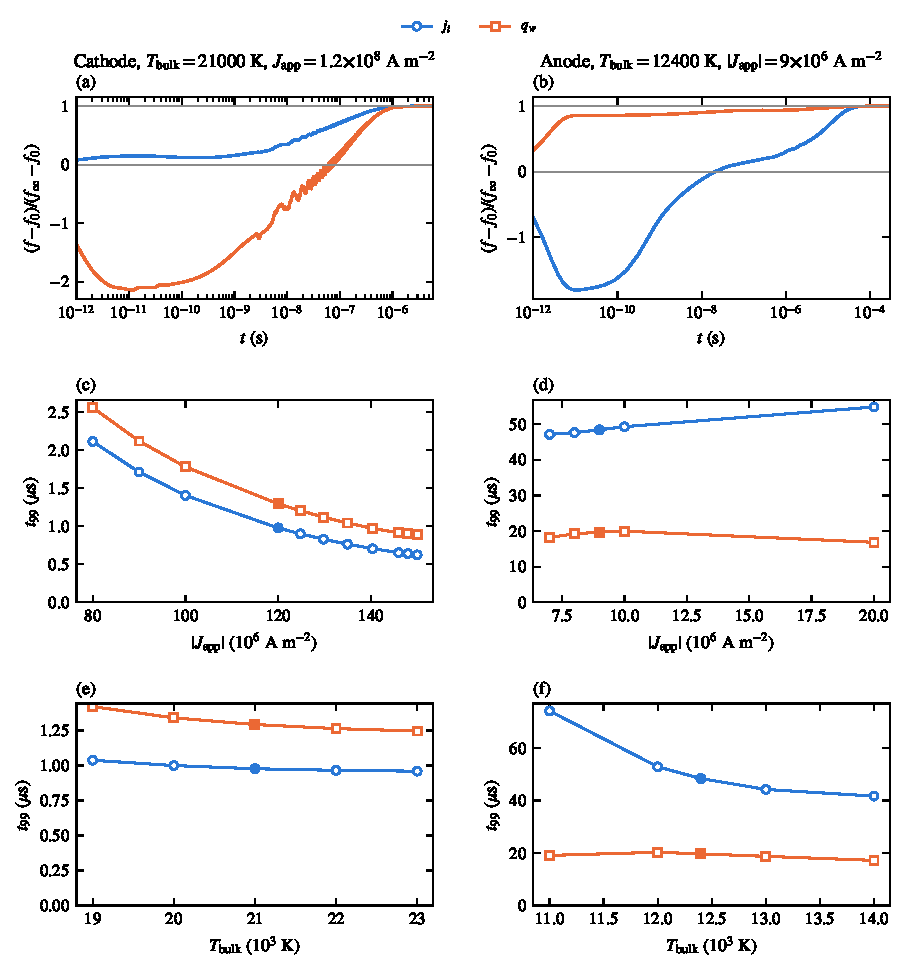
\includegraphics[width=0.92\textwidth]{figures/results_fig/base_timescales.pdf}
\caption{Response of the electrode quantities to a \(+2\,\%\) step of \(|J_{\rm app}|\): cathode (left, axial acoustics removed) and anode (right). Blue: ion current density \(j_i\) at the surface; orange: heat flux \(q_w\) into the surface. (a), (b) Normalized response of the base cases, \(f_0\) and \(f_\infty\) being the initial and the final values. (c), (d) Time to steady state \(t_{99}\) against \(|J_{\rm app}|\) at the base \(T_{\rm bulk}\). (e), (f) \(t_{99}\) against \(T_{\rm bulk}\) at the base \(|J_{\rm app}|\). Filled symbols: the base cases.}
\label{fig:timescales}
\end{figure}

\emph{Cathode.} The response has two stages (figure~\ref{fig:timescales}(a)). About 15\,\% of the change of \(j_i\) occurs within 10~ps; the rest follows within about \(1\ \mu\)s, \(t_{99}=0.98\ \mu\)s, the final approach being exponential with a relaxation time of \(0.29\ \mu\)s. The heat flux first moves in the opposite direction and settles later, \(t_{99}=1.29\ \mu\)s. The cathode layer responds faster at higher current density: between \(8\times10^{7}\) and \(1.5\times10^{8}\ \mathrm{A\,m^{-2}}\), \(t_{99}\) falls from 2.1 to 0.62~\(\mu\)s for \(j_i\) and from 2.6 to 0.89~\(\mu\)s for \(q_w\) (figure~\ref{fig:timescales}(c)). The bulk temperature changes \(t_{99}\) by less than 15\,\% between 19\,000 and 23\,000~K (figure~\ref{fig:timescales}(e)).

\emph{Anode.} The anode layer relaxes about 40 times more slowly, with a relaxation time of \(11\ \mu\)s, and its two quantities behave differently (figure~\ref{fig:timescales}(b)). Because the dominant electron terms of the heat flux~(\ref{eq:bc-qwall}) are carried by the current (Section~\ref{sec:res-heat}), 87\,\% of the change of \(q_w\) occurs within 1~ns, and \(t_{99}=20\ \mu\)s. The ion current density first moves in the opposite direction and needs \(t_{99}=48\ \mu\)s. For \(j_i\), \(t_{99}\) decreases from 74 to 42~\(\mu\)s as \(T_{\rm bulk}\) rises from 11\,000 to 14\,000~K and increases only from 47 to 55~\(\mu\)s over the current range; that of \(q_w\) stays between 17 and \(20\ \mu\)s in all cases (figure~\ref{fig:timescales}(d), (f)).

The cathode layer can therefore be treated as quasi-steady for changes of the arc slower than a few microseconds. At the anode, the heat flux follows the current within about \(20\ \mu\)s, but the ion current needs 40--75~\(\mu\)s.
\clearpage
